\documentclass[12pt]{article}

% ---------- Packages ----------
\usepackage[margin=1in]{geometry}
\usepackage{amsmath, amssymb}
\usepackage{graphicx}
\usepackage{float}        % [H] exact figure placement
\usepackage{placeins}     % \FloatBarrier to stop floats crossing sections
\usepackage{setspace}
\usepackage{hyperref}
\usepackage{caption}      % \captionof if ever needed
\usepackage{booktabs}

\onehalfspacing

% Make LaTeX look for images in ./figures relative to this file
\graphicspath{{figures/}}

% ---------- Metadata ----------
\title{\textbf{A Computational Study of Derivative Pricing under Stochastic Volatility Using the Black--Scholes Framework}}
\author{\textbf{Ekantheswar Bandarupalli}\\
\small Working Paper --- Computational Finance Research\\
\small \texttt{study.ekantheswar@gmail.com}}
\date{\today}

% ---------- PDF meta ----------
\hypersetup{
  colorlinks=true,
  linkcolor=blue,
  citecolor=blue,
  urlcolor=blue,
  pdftitle={A Computational Study of Derivative Pricing under Stochastic Volatility Using the Black--Scholes Framework},
  pdfauthor={Ekantheswar Bandarupalli}
}

\begin{document}
\maketitle

\thispagestyle{empty}

% ---------- Abstract ----------
\begin{abstract}
The intersection of financial markets and mathematical modeling has long fascinated both practitioners and academics.
While algorithmic trading first sparked my interest in finance, it was the underlying question of how risk and price evolve
that drew me toward stochastic calculus and derivative pricing. This study presents a reproducible computational baseline for
pricing European options using the Black--Scholes model and compares theoretical values with real S\&P 500 (SPX) market data.
We highlight model fit, limitations arising from the constant volatility assumption, and outline directions toward stochastic
volatility models such as Heston.
\end{abstract}

\textbf{Keywords:} Black--Scholes, Stochastic Volatility, SPX Options, Greeks, Quantitative Finance


\newpage
\setcounter{page}{1}

% ---------- Introduction ----------
\section{Introduction}
My initial interest in financial markets began through trading, where market behavior seemed both systematic and unpredictable.
What began as an exploration of trading systems evolved into a deeper curiosity about the mathematics governing price movements,
volatility, and risk. I soon realized that true insight lies not in execution alone, but in the stochastic models that shape
financial dynamics. The objective of this work is to bridge theoretical finance with computational implementation.
By applying the Black--Scholes model to real SPX option data, this paper evaluates accuracy, limitations, and potential extensions
toward stochastic volatility.

% ---------- Methodology ----------
\section{Methodology}
The Black--Scholes model, first introduced by Black and Scholes~\cite{black1973pricing}, provides a closed-form framework for pricing European options under assumptions of constant volatility and lognormal asset dynamics. We consider the standard Black--Scholes setting with underlying price $(S_t)_{t\ge 0}$ following geometric Brownian motion under the
risk--neutral measure. Under the risk-neutral framework described in~\cite{black1973pricing}, the asset price $S_t$ is modeled as geometric Brownian motion, leading to closed-form pricing expressions and analytical sensitivities via the Greeks.
\begin{equation}
dS_t = r S_t\,dt + \sigma S_t\, dW_t,
\end{equation}
where $r$ is the constant risk--free rate, $\sigma$ the (assumed constant) volatility, and $(W_t)$ a standard Brownian motion.
For a European call with strike $K$ and maturity $T$, the no--arbitrage price at $t=0$ is
\begin{equation}
C = S_0 \Phi(d_1) - K e^{-rT} \Phi(d_2), \quad
d_{1,2} = \frac{\ln(S_0/K) + (r \pm \tfrac{1}{2}\sigma^2)T}{\sigma\sqrt{T}},
\end{equation}
and for a put
\begin{equation}
P = K e^{-rT} \Phi(-d_2) - S_0 \Phi(-d_1),
\end{equation}
where $\Phi$ denotes the standard normal CDF.

We compute the \emph{Greeks} to assess sensitivities: Delta ($\partial C/\partial S$), Gamma ($\partial^2 C/\partial S^2$),
Vega ($\partial C/\partial \sigma$), Theta ($\partial C/\partial T$), and Rho ($\partial C/\partial r$), using closed--form expressions.
Empirically, we retrieve SPX option chains via public market data, construct time--to--maturity $T$ and strike grids near the
at--the--money (ATM) region, and compare market mid quotes with Black--Scholes prices computed using market implied volatilities.
Pricing errors are reported as (market price $-$ model price).

\paragraph{Limitations.}
The constant volatility assumption induces systematic mispricing patterns (e.g., volatility smile/smirk). In subsequent work we outline
a stochastic volatility extension (Heston) with variance process
$d\nu_t = \kappa(\theta-\nu_t)\,dt + \xi \sqrt{\nu_t}\, dZ_t$ and price via Fourier methods or simulation.

% ---------- Results ----------
\section{Results}
We analyze the nearest--maturity SPX option chain and compare market mid prices with Black--Scholes values computed using market
implied volatilities. Figure~\ref{fig:pricing-error} shows the pricing error across strikes near the ATM region.
We also report illustrative Greek curves (Delta and Gamma) around ATM using a representative maturity and IV.

% --- Figure 1: Pricing Error ---
\begin{figure}[H]
\centering
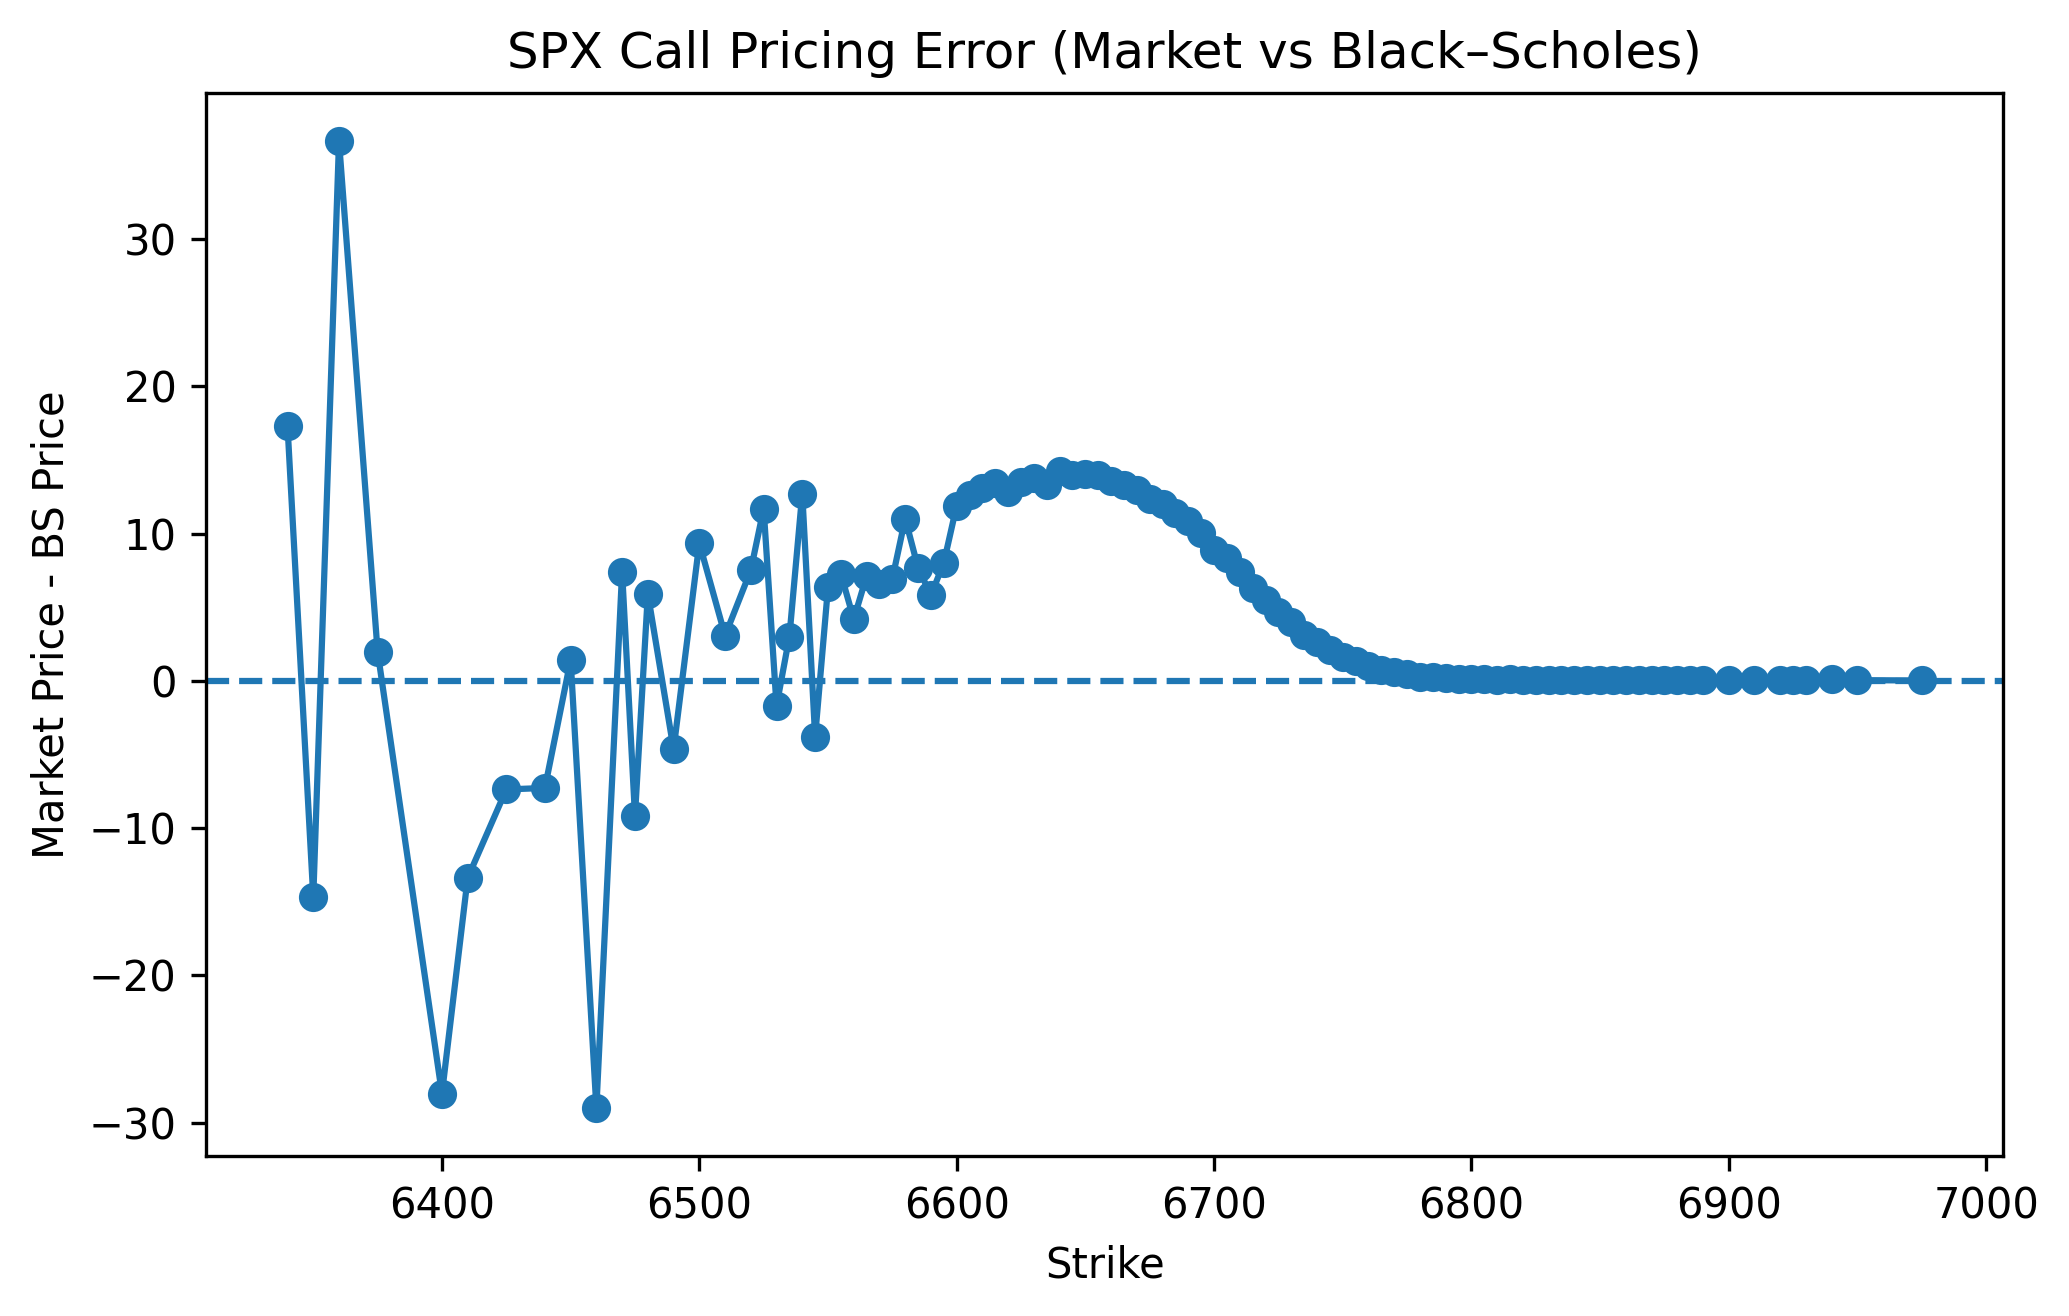
\includegraphics[width=0.85\linewidth]{pricing_error_vs_strike.png}
\caption{Market vs.\ Black--Scholes mispricing by strike for SPX calls near the ATM region and nearest expiry.
Positive values indicate the market is priced above the baseline model.}
\label{fig:pricing-error}
\end{figure}

% --- Figure 2: Delta ---
\begin{figure}[H]
\centering
\includegraphics[width=0.85\linewidth]{delta_vs_strike.png}
\caption{Delta as a function of strike (nearest maturity, representative IV). The transition around ATM reflects
the probability mass under the risk--neutral distribution.}
\label{fig:delta}
\end{figure}

% --- Figure 3: Gamma ---
\begin{figure}[H]
\centering
\includegraphics[width=0.85\linewidth]{gamma_vs_strike.png}
\caption{Gamma as a function of strike (nearest maturity, representative IV). The peak at ATM indicates heightened
curvature (sensitivity of Delta) for short maturities.}
\label{fig:gamma}
\end{figure}

\FloatBarrier % <-- Ensures all figures stay before next section

% ---------- Discussion and Future Work ----------

\section{Discussion and Future Work}

\subsection{Interpretation of Results}
The empirical results highlight systematic discrepancies between market prices and the Black--Scholes baseline, particularly across strikes surrounding the at--the--money region. These deviations are consistent with the well-documented \emph{volatility smile} and \emph{skew} phenomena, where implied volatilities vary by strike rather than remaining constant. In practice, out-of-the-money options often carry higher implied volatilities due to demand for tail-risk protection, while at-the-money options generally reflect more balanced beliefs about short-term uncertainty.

The presence of persistent pricing errors indicates that the constant-volatility assumption of Black--Scholes cannot fully capture market dynamics. Although the model serves as an analytically elegant starting point, its single-parameter volatility framework leads to underestimation or overestimation of option values depending on moneyness. This reinforces the need for richer stochastic models capable of representing time-varying and state-dependent volatility structures.

% ---------- Future Work ----------

\subsection{Future Work: Heston Model}
Future research will extend this analysis using stochastic volatility models. A prominent stochastic volatility framework is the Heston model~\cite{heston1993closed}, in which the variance follows a mean-reverting square-root process correlated with the asset price.
:
\begin{equation}
\begin{aligned}
dS_t &= \mu S_t\,dt + \sqrt{v_t}\, S_t\, dW_t^S, \\
dv_t &= \kappa(\theta - v_t)\,dt + \xi \sqrt{v_t}\, dW_t^v,
\end{aligned}
\end{equation}
where $v_t$ denotes instantaneous variance, $\kappa$ is the rate of mean reversion, $\theta$ the long-run variance, and $\xi$ the volatility of variance. By allowing the volatility to evolve stochastically, the Heston model provides a more flexible framework to capture empirical features such as smile, skew, and term structure. Calibration and comparison against SPX market data will form the basis of future empirical work.




% ---------- Conclusion ----------

\section{Conclusion}
This study implemented the Black--Scholes framework and applied it to real SPX option data to evaluate theoretical pricing under constant volatility assumptions. The observed pricing discrepancies and systematic volatility patterns highlight the limitations of deterministic volatility models in capturing market behavior. By examining Greeks and pricing errors across strikes, we established a computational baseline from which more advanced stochastic volatility frameworks can evolve.

Looking ahead, models such as Heston offer a mathematically richer foundation by allowing volatility itself to vary over time and state. Incorporating such dynamics represents a natural progression of this work and aligns with my broader goal of contributing to financial modeling that is both mathematically rigorous and practically relevant. Ultimately, I aim to bridge mathematical finance and quantitative innovation in industry, building tools and insights that serve both research and real-world applications.

% ---------- Acknowledgment ----------
\section*{Acknowledgment}
This work is part of my independent research initiative in computational finance, conducted in preparation for doctoral studies in Financial Mathematics.


% ---------- References ----------

\bibliographystyle{plain}
\bibliography{references}


\end{document}
